\documentclass[10pt]{article}

\usepackage[letterpaper,margin=0.5in]{geometry}
\usepackage[T1]{fontenc}
\usepackage[scaled=0.95]{helvet}
\renewcommand{\familydefault}{\sfdefault}
\usepackage{microtype}
\usepackage[table]{xcolor}
\usepackage{graphicx}
\usepackage{tabularx}
\usepackage{array}
\usepackage{booktabs}
\usepackage{enumitem}
\usepackage[most]{tcolorbox}
\usepackage{setspace}

% Agency-style palette and document rhythm.
\definecolor{agencyblue}{HTML}{005A8B}
\definecolor{deepsea}{HTML}{143B5D}
\definecolor{labline}{HTML}{A9BBC8}
\definecolor{panelbg}{HTML}{F6F8FA}
\definecolor{titlebg}{HTML}{EAF2F7}
\definecolor{textgray}{HTML}{2F3B45}

\pagecolor{white}
\pagestyle{empty}
\color{textgray}
\setstretch{0.99}
\setlength{\parindent}{0pt}
\setlength{\parskip}{2.5pt}
\setlength{\tabcolsep}{4pt}
\renewcommand{\arraystretch}{1.08}
\setlist[itemize]{leftmargin=1.15em,labelsep=0.5em,itemsep=2pt,topsep=2pt,parsep=0pt}
\setlist[enumerate]{leftmargin=1.25em,labelsep=0.5em,itemsep=2pt,topsep=2pt,parsep=0pt}
\newcolumntype{Y}{>{\raggedright\arraybackslash}X}

\newtcolorbox{labbox}[2][]{
  colback=panelbg,
  colframe=labline,
  colbacktitle=titlebg,
  coltitle=deepsea,
  fonttitle=\bfseries\small,
  title=\MakeUppercase{#2},
  boxrule=0.5pt,
  arc=0pt,
  left=7pt,
  right=7pt,
  top=5pt,
  bottom=5pt,
  toptitle=3pt,
  bottomtitle=3pt,
  #1
}

\begin{document}
\small

\begin{tcolorbox}[
  colback=white,
  colframe=deepsea,
  boxrule=0.9pt,
  arc=0pt,
  left=8pt,
  right=8pt,
  top=8pt,
  bottom=7pt
]
\begin{minipage}[c]{0.17\textwidth}
\centering
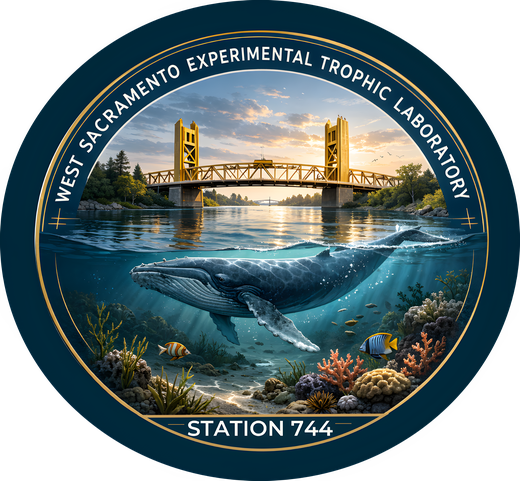
\includegraphics[width=1.00\linewidth]{../images/logo_small.png}
\end{minipage}\hfill
\begin{minipage}[c]{0.78\textwidth}
{\scriptsize\textbf{\color{agencyblue}W.E.T. LAB FIELD OPERATIONS UNIT}}\par
\vspace{2pt}
{\Large\bfseries\color{deepsea}Station 744 Specimen Catalog Survey}\par
\vspace{2pt}
{\small Field Documentation Exercise | Taxonomic Intake Protocol}
\end{minipage}

\vspace{7pt}
{\footnotesize
\rowcolors{1}{titlebg}{white}
\begin{tabularx}{\textwidth}{@{}>{\bfseries\color{deepsea}}l Y >{\bfseries\color{deepsea}}l Y@{}}
Program & Field taxonomy and phenotypic documentation & Status & Internal use only \\
Required gear & Polaroid camera and station notebook & Award & \$250 research funding \\
\end{tabularx}}
\end{tcolorbox}

\vspace{6pt}

\begin{minipage}[t]{0.485\textwidth}
\vspace{0pt}
\begin{labbox}{Study Objective}
Generate a complete catalog record for every lab member using photographic evidence and concise taxonomic notes that would still make sense to another researcher later.
\end{labbox}

\begin{labbox}{Ecological Background}
\begin{itemize}
\item Field biologists often document organisms they cannot collect, preserve, or identify on the spot.
\item A useful catalog entry pairs an image voucher with notes on distinguishing traits and ecological role.
\item Taxonomy turns casual observation into data by standardizing how organisms are described and compared.
\end{itemize}
\end{labbox}

\begin{labbox}{Experimental System}
\begin{itemize}
\item Research lab = collecting team
\item Team member = focal specimen
\item Polaroid = photographic voucher
\item Notebook = field catalog ledger
\item Species name, key trait, and ecological role = minimum metadata standard
\end{itemize}
\end{labbox}

\begin{labbox}{Protocol}
\begin{enumerate}
\item Photograph each team member as an individual specimen.
\item For every specimen, create a notebook entry with a photo or clear photo identifier, a species name, one key trait, and one ecological role.
\item Use observable morphology, behavior, or habitat logic rather than vague inside jokes.
\item Compare catalogs for completeness: one valid entry per team member wins. Ties go to the lab with clearer diagnostic traits and more coherent ecological roles.
\end{enumerate}
\end{labbox}
\end{minipage}\hfill
\begin{minipage}[t]{0.485\textwidth}
\vspace{0pt}
\begin{labbox}{Required Record Fields}
\begin{tabularx}{\linewidth}{@{}>{\bfseries}l Y@{}}
\toprule
Field & Why it matters \\
\midrule
Photo voucher & Preserves evidence of the observed specimen \\
Species name & Establishes a label for comparison and discussion \\
Key trait & Identifies the diagnostic feature that separates this organism from others \\
Ecological role & Connects the specimen to a food web or habitat function \\
\bottomrule
\end{tabularx}
\end{labbox}

\begin{labbox}{Scientific Relevance}
This station mirrors real museum, survey, and biodiversity workflows. Researchers routinely use photographs plus metadata to document unusual individuals, track phenotypic variation, and build records for later identification. Requiring an ecological role keeps the catalog tied to function, not just appearance, which is how field observations become useful biological evidence.
\end{labbox}

\begin{labbox}{Field Note Standards}
\begin{itemize}
\item Strong traits are specific: elongated snout, filter-feeding mouth, defensive spines, bioluminescent lure.
\item Strong ecological roles fit marine systems: grazer, ambush predator, scavenger, parasite, habitat engineer.
\item Better entries distinguish similar specimens by what another observer could actually verify.
\item A complete, legible record matters more than a glamorous photo alone.
\end{itemize}
\end{labbox}

\begin{labbox}{Observational Notes}
Monitor whether the lab creates coherent species concepts across all members, uses diagnostic terminology consistently, and matches traits to plausible trophic or habitat roles.
\end{labbox}
\end{minipage}

\vspace{6pt}

\begin{labbox}{Outcome}
Winning lab demonstrates \textbf{superior field documentation, taxonomic reasoning, and ecological interpretation of novel specimens}. Award disbursement: \textbf{\$250 research funding}.

\vspace{3pt}
\textbf{Completion bonus reminder:} labs that complete all mini-games earn an additional \textbf{+\$100}.
\end{labbox}

\vfill
\begin{center}
\footnotesize\color{agencyblue}\textbf{W.E.T. LAB | Station 744 | Internal Use Only}
\end{center}

\end{document}
